\documentclass{beamer}
\usepackage{tikz}
\usetikzlibrary{arrows.meta, positioning}

\begin{document}

\begin{frame}{Bounded Morphism Illustration}
\centering
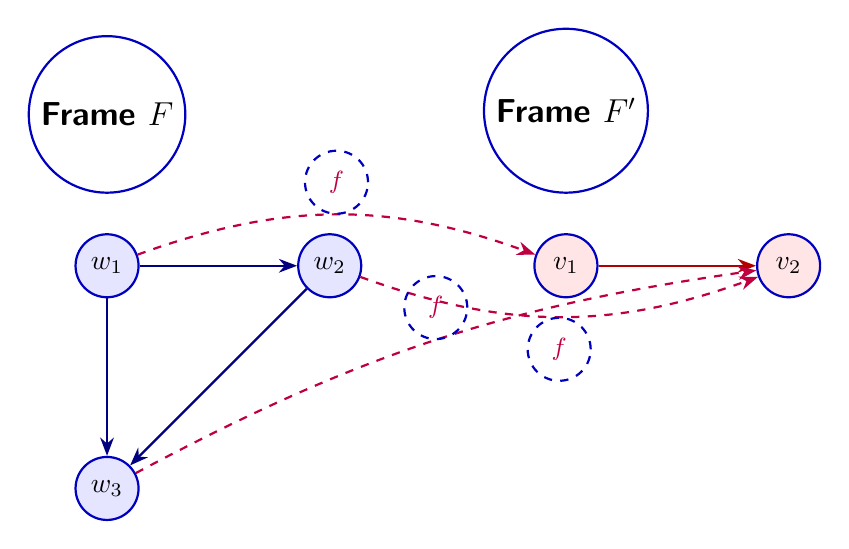
\begin{tikzpicture}[>=Stealth, node distance=2cm, every node/.style={circle, draw=blue!75!black, thick, minimum size=8mm, font=\sffamily\bfseries}]

% Left frame F
\node[fill=blue!10] (w1) {$w_1$};
\node[fill=blue!10, right=of w1] (w2) {$w_2$};
\node[fill=blue!10, below=of w1] (w3) {$w_3$};

% Arrows in F
\draw[->, thick, blue!50!black] (w1) -- (w2);
\draw[->, thick, blue!50!black] (w2) -- (w3);
\draw[->, thick, blue!50!black] (w1) -- (w3);

% Right frame F'
\node[fill=red!10, right=5cm of w1] (v1) {$v_1$};
\node[fill=red!10, right=of v1] (v2) {$v_2$};

% Arrows in F'
\draw[->, thick, red!70!black] (v1) -- (v2);

% Mapping f (dashed arrows)
\draw[->, dashed, thick, purple] (w1) to[bend left=20] node[above]{\small $f$} (v1);
\draw[->, dashed, thick, purple] (w2) to[bend right=20] node[below]{\small $f$} (v2);
\draw[->, dashed, thick, purple] (w3) to[bend left=10] node[above]{\small $f$} (v2);

% Labels for frames
\node[above=0.5cm of w1, font=\sffamily\bfseries\large] {Frame $F$};
\node[above=0.5cm of v1, font=\sffamily\bfseries\large] {Frame $F'$};

\end{tikzpicture}
\end{frame}

\end{document}